\element{CONV4.Presentation}{
  \begin{questionmult}{presentationContinue}\bareme{haut=2,p=0}
    Parmi les propositions ci-dessous, lesquelles sont en présentation continue.
    \begin{multicols}{2}
      \begin{reponses}
        \bonne{$u=0$, $i=cte$}
        \bonne{$u=cte$, $i=0$}
        \bonne{$u=cte$, $i=cte$}
        \bonne{$u=1+4\cos(\omega t)$, $i=3\cos(\omega t)$}
        \bonne{$u=4\cos(\omega t)$, $i=4+3\cos(\omega t)$}
        \mauvaise{$u=4\cos(\omega t)$, $i=3\cos(\omega t)$}
        \mauvaise{$u=4\cos(\omega t)$, $i=0$}
      \end{reponses}
    \end{multicols}
  \end{questionmult}
}
\element{CONV4.Presentation}{
  \begin{questionmult}{presentationAlternative}\bareme{haut=2,p=0}
    Parmi les propositions ci-dessous, lesquelles sont en présentation alternative.
    \begin{multicols}{2}
      \begin{reponses}
        \mauvaise{$u=0$, $i=cte$}
        \mauvaise{$u=cte$, $i=0$}
        \mauvaise{$u=cte$, $i=cte$}
        \mauvaise{$u=1+4\cos(\omega t)$, $i=3\cos(\omega t)$}
        \mauvaise{$u=4\cos(\omega t)$, $i=4+3\cos(\omega t)$}
        \bonne{$u=4\cos(\omega t)$, $i=3\cos(\omega t)$}
        \bonne{$u=4\cos(\omega t)$, $i=0$}
      \end{reponses}
    \end{multicols}
  \end{questionmult}
}
\setgroupmode{CONV4.Presentation}{cyclic}

\element{CONV4.OdG}{
  \begin{question}{puissanceCharbon}\bareme{1}
    L'ordre de grandeur de la puissance délivrée par une centrale au charbon est
    \begin{multicols}{2}
      \begin{reponses}
        \bonne{\SI{1e8}{W}}
        \mauvaise{\SI{1e6}{W}}
        \mauvaise{\SI{1e4}{W}}
        \mauvaise{\SI{1e2}{W}}
      \end{reponses}
    \end{multicols}
  \end{question}
}
\element{CONV4.OdG}{
  \begin{question}{puissanceEolienne}\bareme{1}
    L'ordre de grandeur de la puissance délivrée par une éolienne est
    \begin{multicols}{2}
      \begin{reponses}
        \mauvaise{\SI{1e8}{W}}
        \bonne{\SI{1e6}{W}}
        \mauvaise{\SI{1e4}{W}}
        \mauvaise{\SI{1e2}{W}}
      \end{reponses}
    \end{multicols}
  \end{question}
}
\setgroupmode{CONV4.OdG}{cyclic}

\element{CONV4.Composition}{
  \begin{questionmult}{compositionConvertisseur}\bareme{haut=2,p=0}
    Un convertisseur idéal peut contenir
    \begin{multicols}{2}
      \begin{reponses}
        \bonne{des diodes}
        \bonne{des transistors}
        \bonne{des interrupteurs}
        \bonne{des bobines}
        \bonne{des condensateurs}
      \end{reponses}
    \end{multicols}
  \end{questionmult}
}
\setgroupmode{CONV4.Composition}{cyclic}

\element{CONV4.caractéristique}{
  \begin{questionmult}{caracteristiqueDiode}\bareme{haut=1,p=0}
    Une diode a pour caractéristique
    \begin{multicols}{5}
      \begin{reponses}
        \bonne{
          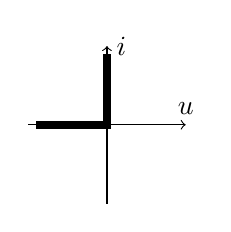
\begin{tikzpicture}
            \draw[->] (-1,0) -- (1,0) node[above] {$u$};
            \draw[->] (0,-1) -- (0,1) node[right] {$i$};
            \draw[line width=1mm] (-0.9,0) -- (0,0) -- (0,0.9);
          \end{tikzpicture}
        }
        \mauvaise{
          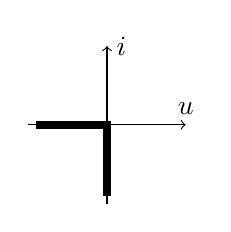
\begin{tikzpicture}
            \draw[->] (-1,0) -- (1,0) node[above] {$u$};
            \draw[->] (0,-1) -- (0,1) node[right] {$i$};
            \draw[line width=1mm] (-0.9,0) -- (0,0) -- (0,-0.9);
          \end{tikzpicture}
        }
        \mauvaise{
          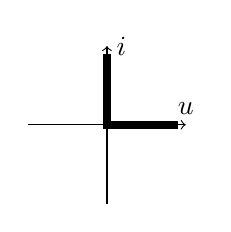
\begin{tikzpicture}
            \draw[->] (-1,0) -- (1,0) node[above] {$u$};
            \draw[->] (0,-1) -- (0,1) node[right] {$i$};
            \draw[line width=1mm] (0.9,0) -- (0,0) -- (0,0.9);
          \end{tikzpicture}
        }
        \bonne{
          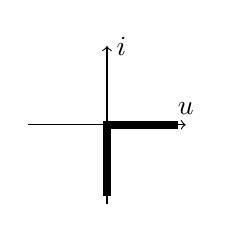
\begin{tikzpicture}
            \draw[->] (-1,0) -- (1,0) node[above] {$u$};
            \draw[->] (0,-1) -- (0,1) node[right] {$i$};
            \draw[line width=1mm] (0.9,0) -- (0,0) -- (0,-0.9);
          \end{tikzpicture}
        }
      \end{reponses}
    \end{multicols}
  \end{questionmult}
}
\element{CONV4.caractéristique}{
  \begin{questionmult}{caracteristiqueTransistor}\bareme{haut=1,p=0}
    Un transistor a pour caractéristique
    \begin{multicols}{4}
      \begin{reponses}
        \mauvaise{
          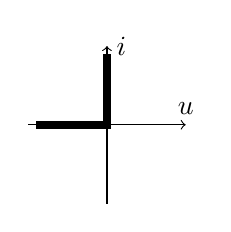
\begin{tikzpicture}
            \draw[->] (-1,0) -- (1,0) node[above] {$u$};
            \draw[->] (0,-1) -- (0,1) node[right] {$i$};
            \draw[line width=1mm] (-0.9,0) -- (0,0) -- (0,0.9);
          \end{tikzpicture}
        }
        \bonne{
          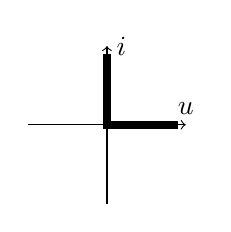
\begin{tikzpicture}
            \draw[->] (-1,0) -- (1,0) node[above] {$u$};
            \draw[->] (0,-1) -- (0,1) node[right] {$i$};
            \draw[line width=1mm] (0.9,0) -- (0,0) -- (0,0.9);
          \end{tikzpicture}
        }
        \mauvaise{
          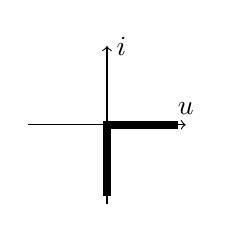
\begin{tikzpicture}
            \draw[->] (-1,0) -- (1,0) node[above] {$u$};
            \draw[->] (0,-1) -- (0,1) node[right] {$i$};
            \draw[line width=1mm] (0.9,0) -- (0,0) -- (0,-0.9);
          \end{tikzpicture}
        }
      \end{reponses}
    \end{multicols}
  \end{questionmult}
}
\setgroupmode{CONV4.caractéristique}{cyclic}

\element{CONV4.exercice}{
  \begin{questionmult}{exerciceHacheur}\bareme{haut=2,p=0}
    On étudie le hacheur schématisé ci-dessous. Le rapport cyclique est noté $\alpha$.
    \begin{center}
      \begin{circuitikz}
        \draw
          (0,0) to[switch,l_=$K_1$,i>^=$i_e$] (3,0) to[short,i=$i_s$] (5,0) to[european current source] (5,-2) -- (0,-2) to[V,l^=$E$,v_=$u_e$] (0,0)
          (3,-2) to[switch,l=$K_2$,*-*] (3,0)
          (4,-2) to[open,v=$u_s$] (4,0);
      \end{circuitikz}
    \end{center}
    \begin{multicols}{2}
      \begin{reponses}
        \bonne{Les interrupteurs ont un fonctionnement complémentaire.}
        \mauvaise{Les interrupteurs sont soit tous les deux ouverts soit tous les deux fermés.}
        \bonne{$K_1$ est un transistor.}
        \bonne{$K_2$ est une diode.}
        \mauvaise{$K_1$ est une diode.}
        \mauvaise{$K_2$ est un transistor.}
        \bonne{La tension de sortie moyenne vaut $\alpha E$.}
        \mauvaise{Le courant moyen de sortie vaut $\alpha I$.}
      \end{reponses}
    \end{multicols}
  \end{questionmult}
}
\element{CONV4.exercice}{
  \begin{questionmult}{exerciceOnduleur}\bareme{haut=2,p=0}
    On étudie l'onduleur schématisé ci-dessous.
    \begin{center}
      \begin{circuitikz}
        \draw
          (0,0) -- (1,0) to[nos,l_=$K_1$,i>^=$i_1$,*-*] (1,-2) to[nos,l_=$K_4$,i^<=$i_4$,*-*] (1,-4) -- (0,-4) to[V=$E$,i^>=$i_e$] (0,0)
          (1,0) -- (3,0) to[nos,l=$K_2$,i<=$i_2$,-*] (3,-2) to[nos,l=$K_3$,i>=$i_3$] (3,-4) -- (1,-4)
          (1,-2) to[I=$I$,v<=$u$] (3,-2);
      \end{circuitikz}
    \end{center}
    \begin{multicols}{2}
      \begin{reponses}
        \bonne{OFOF est un état possible.}
        \mauvaise{OFFO est un état possible.}
        \mauvaise{FFOO permet de transférer de la puissance entre la source et la charge.}
        \bonne{FOFO permet de de transférer de la puissance entre la source et la charge.}
        \bonne{La tension $u$ vaut soit $E$ soit $-E$.}
        \mauvaise{La présentation d'entrée est alternative.}
      \end{reponses}
    \end{multicols}
  \end{questionmult}
}
\setgroupmode{CONV4.exercice}{cyclic}